\documentclass[conference]{IEEEtran}

% *** GRAPHICS RELATED PACKAGES ***
%
\ifCLASSINFOpdf
   \usepackage[pdftex]{graphicx}
  % declare the path(s) where your graphic files are
  % \graphicspath{{../pdf/}{../jpeg/}}
  % and their extensions so you won't have to specify these with
  % every instance of \includegraphics
   \DeclareGraphicsExtensions{.pdf,.jpeg,.png}
\else
  % or other class option (dvipsone, dvipdf, if not using dvips). graphicx
  % will default to the driver specified in the system graphics.cfg if no
  % driver is specified.
   \usepackage[dvips]{graphicx}
  % declare the path(s) where your graphic files are
   \graphicspath{{../eps/}}
  % and their extensions so you won't have to specify these with
  % every instance of \includegraphics
   \DeclareGraphicsExtensions{.eps}
\fi

% *** MATH PACKAGES ***
%
\usepackage{amsmath,bm,caption}
%\captionsetup{margin=20pt,format=hang,justification=justified}
\usepackage[caption=false,font=footnotesize]{subfig}
\usepackage{natbib}


\usepackage{authblk}
\usepackage[pdfborder={0 0 0}]{hyperref}% For email addresses

\title{Human Activity Recognition Based on Accelerometer and Gyroscope Data}

\author[1]{Junle Lu}
\author[2]{Haomiao Meng}
\author[2]{Xin Qi}

\affil[1]{Department of Electrical and Computer Engineering}
\affil[2]{Department of Mathematical Sciences \protect\\
          State University of New York at Binghamton\\ NY 13905 \protect\\}

\begin{document}

\maketitle

% As a general rule, do not put math, special symbols or citations
% in the abstract
\begin{abstract}
In this paper, we aim to analyze and perform human activity classification based on a published dataset recorded from tri-axial accelerometer and gyroscope sensors. The dataset contains raw sensor readings and includes 561 pre-processed features for human activity classification. Principle component analysis and factor analysis are utilized to visualize and gain more insight into the dataset. The subject effect is determined by using Analysis of Variance (ANOVA) test on each feature. With these exploratory techniques, we have significantly reduced the number of features before classification. Multicategory logistic regression model, multiclass support vector machine (SVM), and random forest are proposed and implemented for human activity classification task. As a result, the support vector machine achieved the best performance with test error 3.8$\%$.\\                                                                                                                
\end{abstract}
\renewcommand\IEEEkeywordsname{Keywords}

\begin{IEEEkeywords}
accelerometer,
gyroscope,
human activity recongnition,
logistic regression,
random forest,
support vector machine
\end{IEEEkeywords}

\section{Introduction}
Human activity recognition (HAR) nowadays become an active research field due to its substantial contributions in human-centered areas of studies. The medical, military and security applications have shown high interests in HAR system \cite{bayat2014study,hamalainen2011jerk}. For instance, a patient with heart problem may require limited daily activities. The HAR system can alert the patient to take a rest in real-time. It also precisely records the patient's activities for diagnosis purpose \cite{kwapisz2011activity}. The HAR system designs are centered around two approaches, namely using external and wearable sensors. For external sensor, the computer vision based techniques have shown promising results for human activity tracking such as Xbox Kinect. However, most of these techniques require infrastructure support \cite{lara2013survey, wuhuman}. Pervasive sensing and computing have become feasible with the recent progress in wearable technology such as Apple Watch. However, recognizing complex activities on light-weight devices is still a challenging task \cite{lara2013survey}. In general, the HAR system have the following three requirements:

\begin{enumerate}
\item Real-time and features are computable in real time.
\item Short sample window duration must be employed to avoid delay response.
\item The classification scheme should be light weight and computational inexpensive.\\
\end{enumerate}

For fulfilling these requirements, many studies have used accelerometer and gyroscope embedded in the wearable devices \cite{bayat2014study,kwapisz2011activity,lara2013survey,wuhuman}. Typically, these sensors are used for obtaining the orientation of the attached object. A tri-axial accelerometer returns a real valued estimate of acceleration along the x, y, and z axes including the gravity. The velocity and displacement can also be estimated from the acceleration. Similarly, the gyroscope returns a real valued estimate of angular velocity along the x, y, and z axes. The accelerometer has shortcomings in dynamic body movements, and the gyroscope has issues such as parameter drifting. Thus, the sensor fusion of accelerometer and gyroscope has been popular for the best estimate of the object's orientation. These sensors are widely available in consumer wearable electronics. In this study, the raw dataset is generated from a smartphone attached to the participant's waist. 

The majority of the smartphones are embedded with tri-axial accelerometer and gyroscope sensors which are crucial for the HAR system. In most smartphones, these sensors are primarily used for automatic screen rotation and indirect user control by detecting the phone's orientation as user inputs. The processing power of the smartphones is more than enough to implement HAR system. In particular, this dataset was generated based on the sensor readings from a Samsung Galaxy II smartphone.

The rest of the paper is organized as follows. In Section II, we introduce the dataset and review some key features. In Section III, we perform exploratory data analysis on the 561 features which are given in the dataset. In Section IV, we present mathematical details about the three proposed classification algorithms. In Section V, the classification algorithms are evaluated with cross validation and their performances are discussed. Finally, the conclusions are given in Section VI. 

\section{Data Summary}
\subsection{Overview}
The dataset is owned by Smartlab and obtained from the UCI machine learning repository. The raw data were collected from a Samsung Galaxy II smartphone with built-in tri-axial accelerometer and gyroscope sensors. In each experiment, the participant was asked to perform a protocol of 12 activities but we are tasked to recognize these six basic activities: standing (ST), sitting (SI), lying (LD), walking (WK), walking downstairs (WD) and walking upstairs (WU). The raw data from the accelerometer and gyroscope are shown in Figure 1 for one experiment. The upper panel is the time series for accelerometer measurement and the lower panel is the time series for gyroscope measurement. It can be seen that different segments have different values and variations, indicating that the person is in different statuses.

\begin{figure}[!ht]
\centering
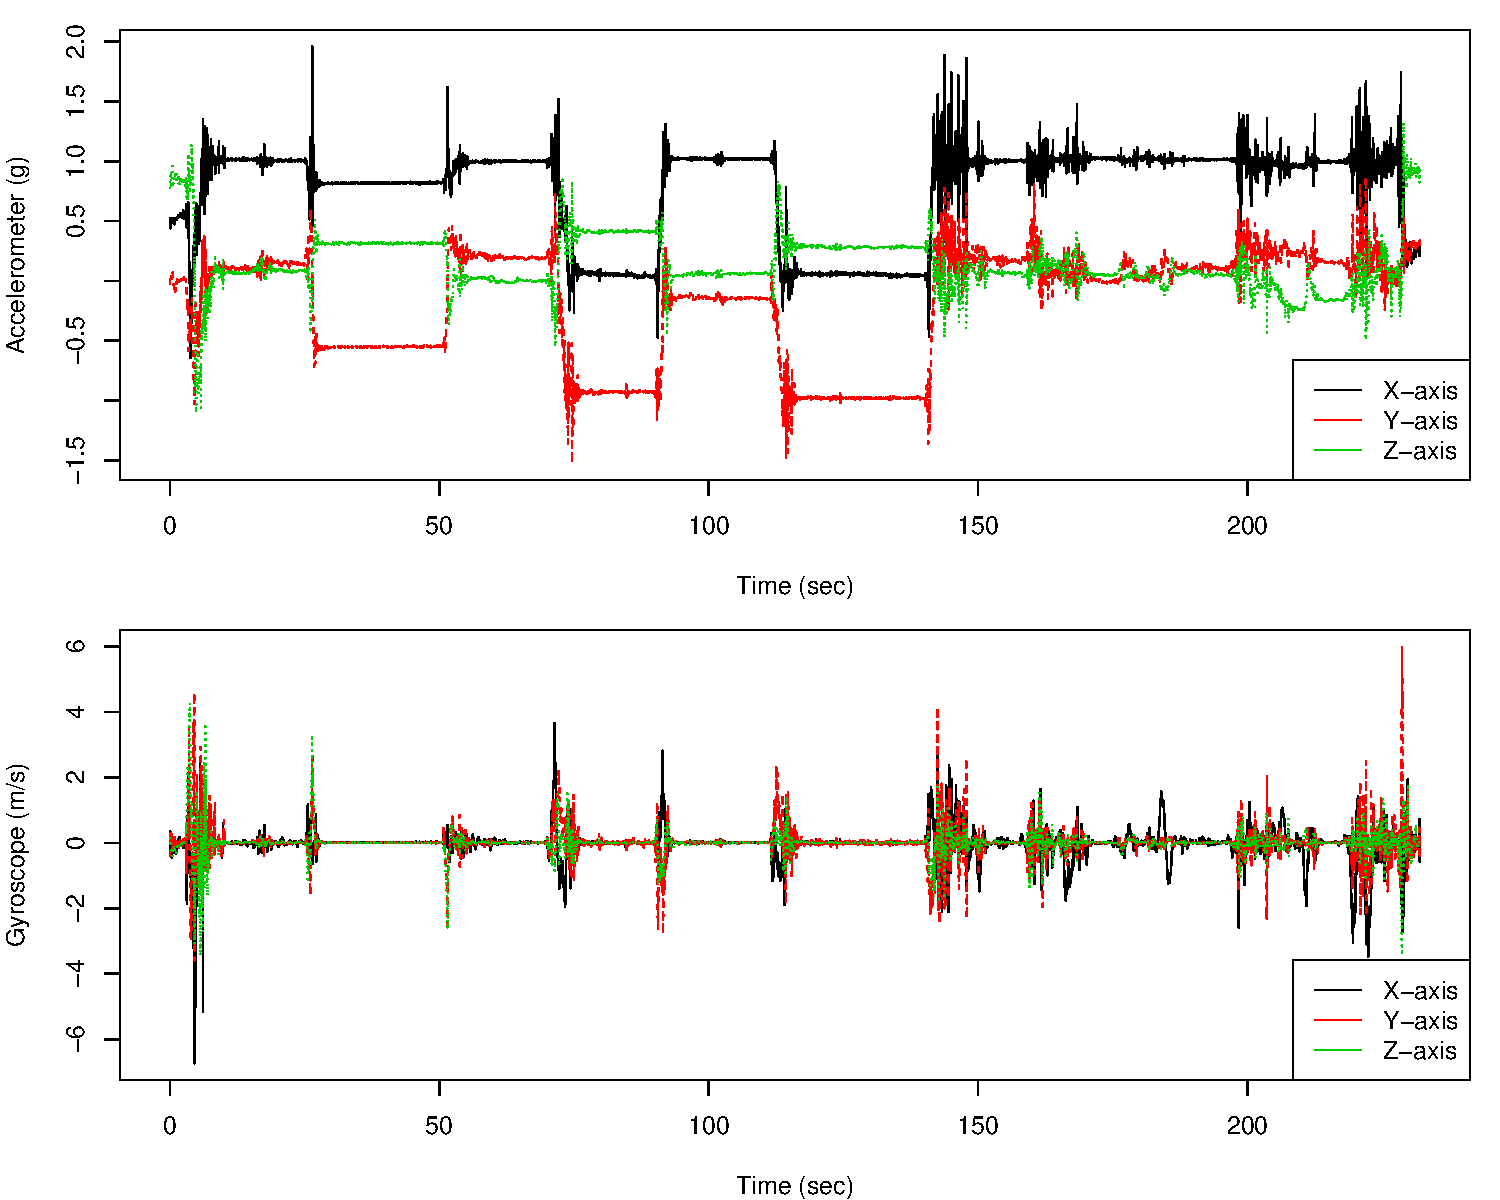
\includegraphics[width=3.2in]{figure1.pdf}
\caption{One participant's raw data in an experiment. The upper panel is for accelerometer data and the lower panel is for gyroscope data.
}
\label{fig_sim}
\end{figure}

Although there is a noticeable difference in original time series for different activities, it is still difficult to distinguish them by using the raw data. For a more practical application, the further processing is required on the raw data to extract useful information related to the six human activities. In \cite{ortiz2015smartphone}, the raw data were collected with the de facto standard in the HAR system research. Specifically, the sensor readings were pre-processed by applying noise filters and then sampled in fixed-width sliding windows of 2.56 seconds and 50$\%$  overlap (128 readings/window). For each 2.56 seconds sample window, 561 features were extracted including frequency domain features.

\subsection{Feature Extraction}
There are total of 10411 sample windows (observations) were generated for 30 participants. About 70$\%$ of them will be used as training set (21 participants). Each sample window was labeled with its human activity and the participant. Moreover, there are 561 features that can be extracted by processing the 6 raw data from the tri-axial accelerometer and gyroscope. By utilizing these features, we should able to distinguish the six different human activities. For those features, they can be classified into 18 categories as shown in Table I.

\begin{table}[htbp]
% increase table row spacing, adjust to taste
\renewcommand{\arraystretch}{1.3}
\caption{Categories of features}
\label{Categories of features}
\centering
\begin{tabular}{|c||c|}
\hline
tBodyAcc (41)&tGravityAccMag (13) \\
\hline
fBodyGyro (79)& tGravityAcc (40) \\
\hline
tBodyAccJerkMag (13)&fBodyAccMag (13)\\
\hline
tBodyAccJerk (41)&tBodyGyroMag (13) \\
\hline
fBodyAccJerkMag (13)& tBodyGyro (41) \\
\hline
tBodyGyroJerkMag (13)& fBodyGyroMag (13)\\
\hline
tBodyGyroJerk (41)& fBodyAcc (79) \\
\hline
fBodyGyroJerkMag (13)& tBodyAccMag (13)\\
\hline
fBodyAccJerk (79)& tAxisAcc (3)\\
\hline
\end{tabular}
\end{table}
					
In Table I, the prefix "t" denotes for time domain signal and the prefix "f" stands for frequency domain signal. Each category includes a set of variables, such as mean, standard deviation, median, auto-regression coefficients and so on. The number of features in each category is denoted in the brackets behind those categories. It is expected that the classification accuracy and computational cost are inversely proportional to the number of the features. However, it is not necessary to use all the features for classification. There are strong and weak features for different activities. By selecting a few features could possibly be sufficient to perform desired classification task. In this particular dataset, different features are more or less used for human activity classification in other work. In other words, it is a collection of feasible features for human activity recognition. Therefore, it is necessary to further analyze these features.

\section{Exploratory Feature Analysis}
\subsection{Subject Effect}
Since the training and testing datasets consist different participants, we need to investigate the subject effect in this case. Sometimes the difference between people (subject effect) is more significant than human activities, which makes it difficult for classification. In order to investigate this subject effect, we perform an ANOVA test on subjects (21 levels) for each feature in the training dataset. As a result, more than 93$\%$ of the tests have p-value less than 0.01, indicating that different individual has different values on those features. 

However, we also notice that even though most of p-values are small, there is still a large difference between dynamic and static activities as shown in Figure 2. This indicates that subject effect is stronger in dynamic than in static activities. In static activities with no human motion, there are 15 features with large subject effect. These features are all related to gravity force measured by the accelerometer such as ”tGravityAcc-Mean-1”. It could mean that the accelerometer is not calibrated for each participant in the experiments. As the sensor is placed on the waist, the accelerometer could be placed slightly different between each participant which may cause inconsistency in the gravity force reading. 

However, there are still some features with small subject effects. These features are mean value of the body components from sensor readings such as ”tBodyAcc-Mean- 1”. This may imply that different activities may have unique characteristic in sensor readings. 

\begin{figure}[!ht]
\centering
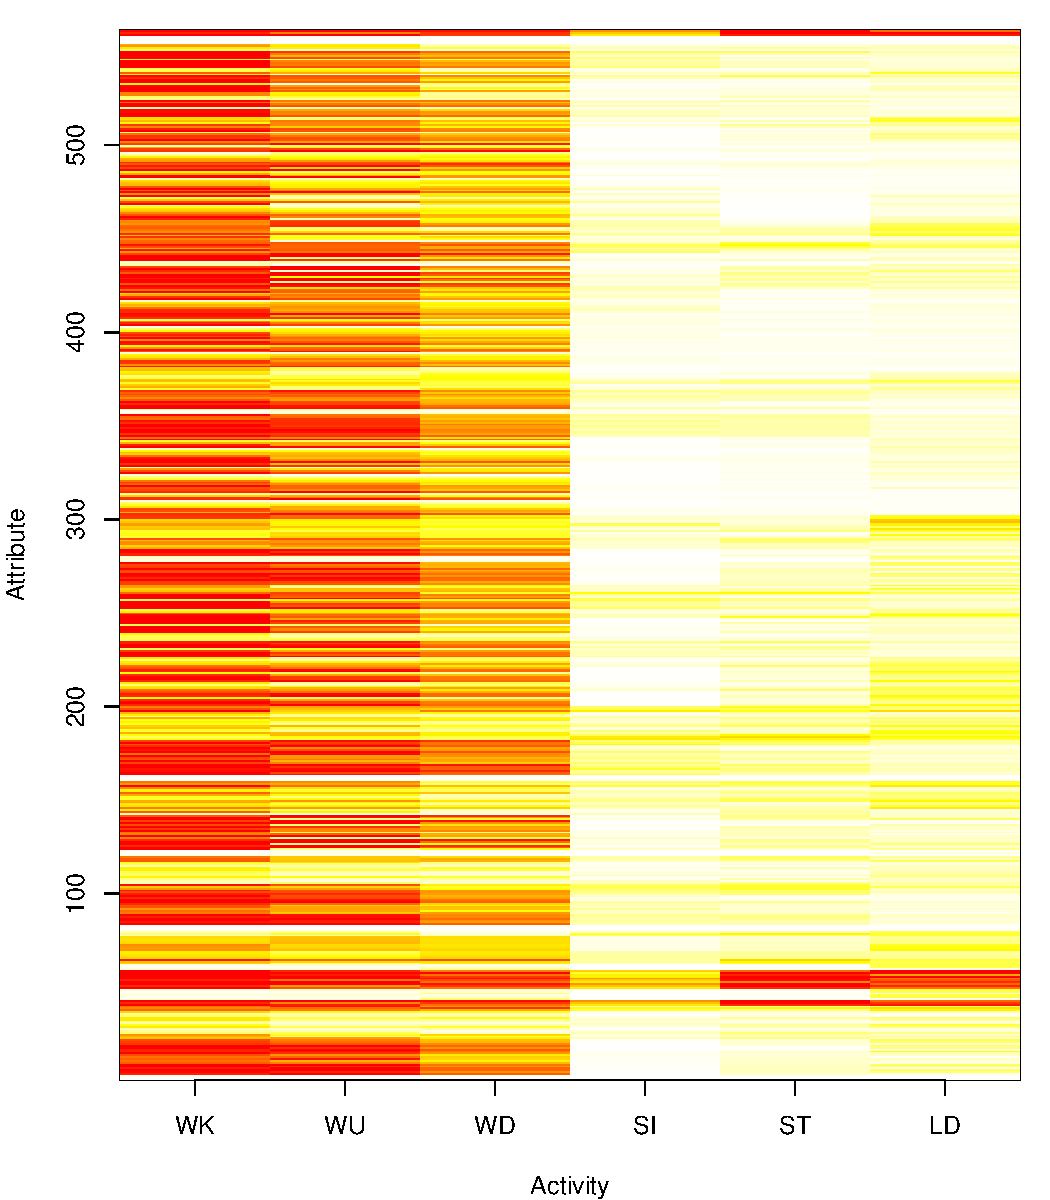
\includegraphics[width=2.8in]{figure2.pdf}
\caption{Log p-value for testing subject effect in each feature (Y-axis) and each activity (X-axis). The subject effect is proportional to the intensity of the color.
}
\label{fig_sim}
\end{figure}

Although there is a large subject effect, a good classifier can still be built if there is a greater activity effect. We perform a two-way ANOVA for each feature to compare the activity effect with subject effect. Typically, a two-way ANOVA decomposition can be written as:
$$SSTO=SSA+SSB+SSAB+SSE$$
Here, SSTO is the total sum of square, SSA is the sum of square of effect A, SSB is the sum of square of effect B, SSAB is the sum of square of interaction, and SSE stands for the sum of square of error. Then we define the relative strength of effect A and effect B as:
$$r=\frac{SSA/df_{A}}{SSB/df_{B}}$$
We find 258 features with $r>10$ and 85 features with $r>30$. This implies that a large number of variables can be chosen to overcome subject effect. However, there are also 32 features with $r<1$, which means activity effect is not stronger than subject effect. Four variables are chosen to display the relationship between subject effect and activity effect in Figure 3. The upper left panel is a variable that separates dynamic activities and static activities, as well as walking downstairs and other two dynamic activities; the upper right panel is a variable that separates walking upstairs with other activities; the bottom left panel is a variable that separates static activities; and the bottom right panel is a variable with larger subject effect than activity effect (a variable trying to avoid to use).

\begin{figure}[!ht]
\centering
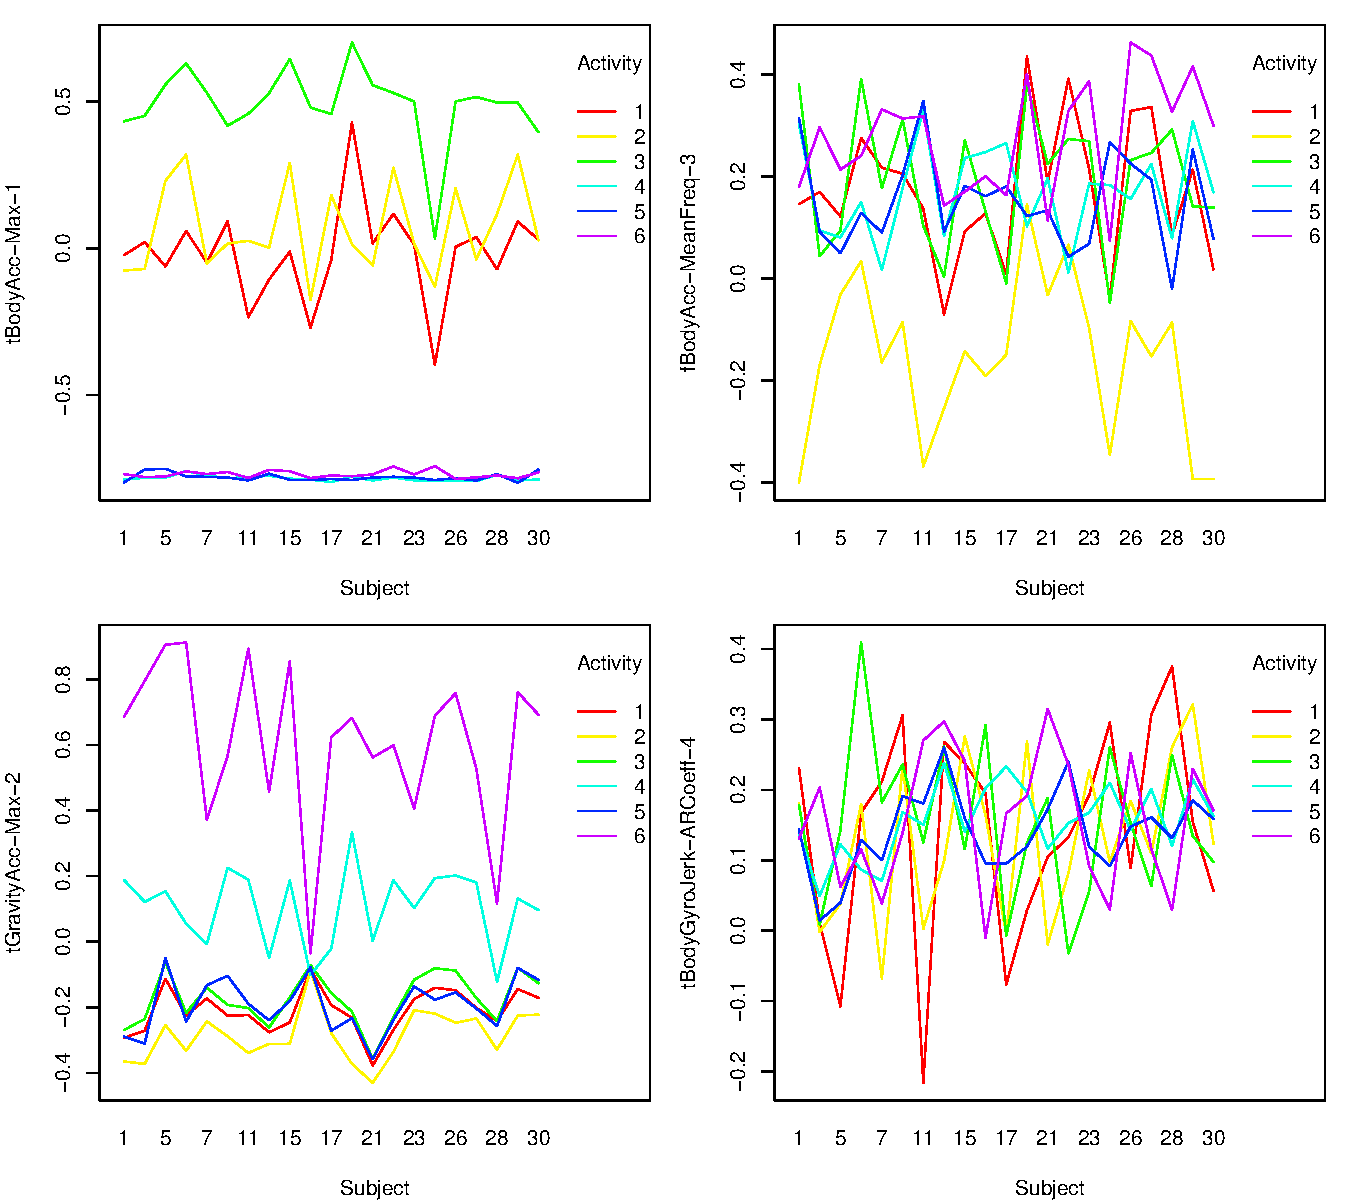
\includegraphics[width=3.2in]{figure3.pdf}
\caption{Interaction plot for four features. Each point stands for the mean value of the feature on each subject (X-axis) and each activity (different lines). 1=WK, 2=WU, 3=WD, 4=SI, 5=ST and 6=LD.
}
\label{fig_sim}
\end{figure}

\subsection{Principle Component Analysis}
From data pre-processing, we expect there exists strong correlations between some features. For instance, the “jerk” signal (tBodyAccJerk) is the time derivative of the acceleration signal (tBodyAcc). Moreover, there are 561 features in the dataset, which are difficult to interpret. Thus, we implement principle component analysis (PCA) to reduce the dimension of variables.

Figure 4 shows the scatter plot for the first three PC scores. From this plot, we find that the first PC clearly splits the six activities into dynamic and static status. The second PC along with the first PC could help to explain the difference in dynamic status, while the third PC is mainly for distinguishing different static status. 

\begin{figure}[!ht]
\centering
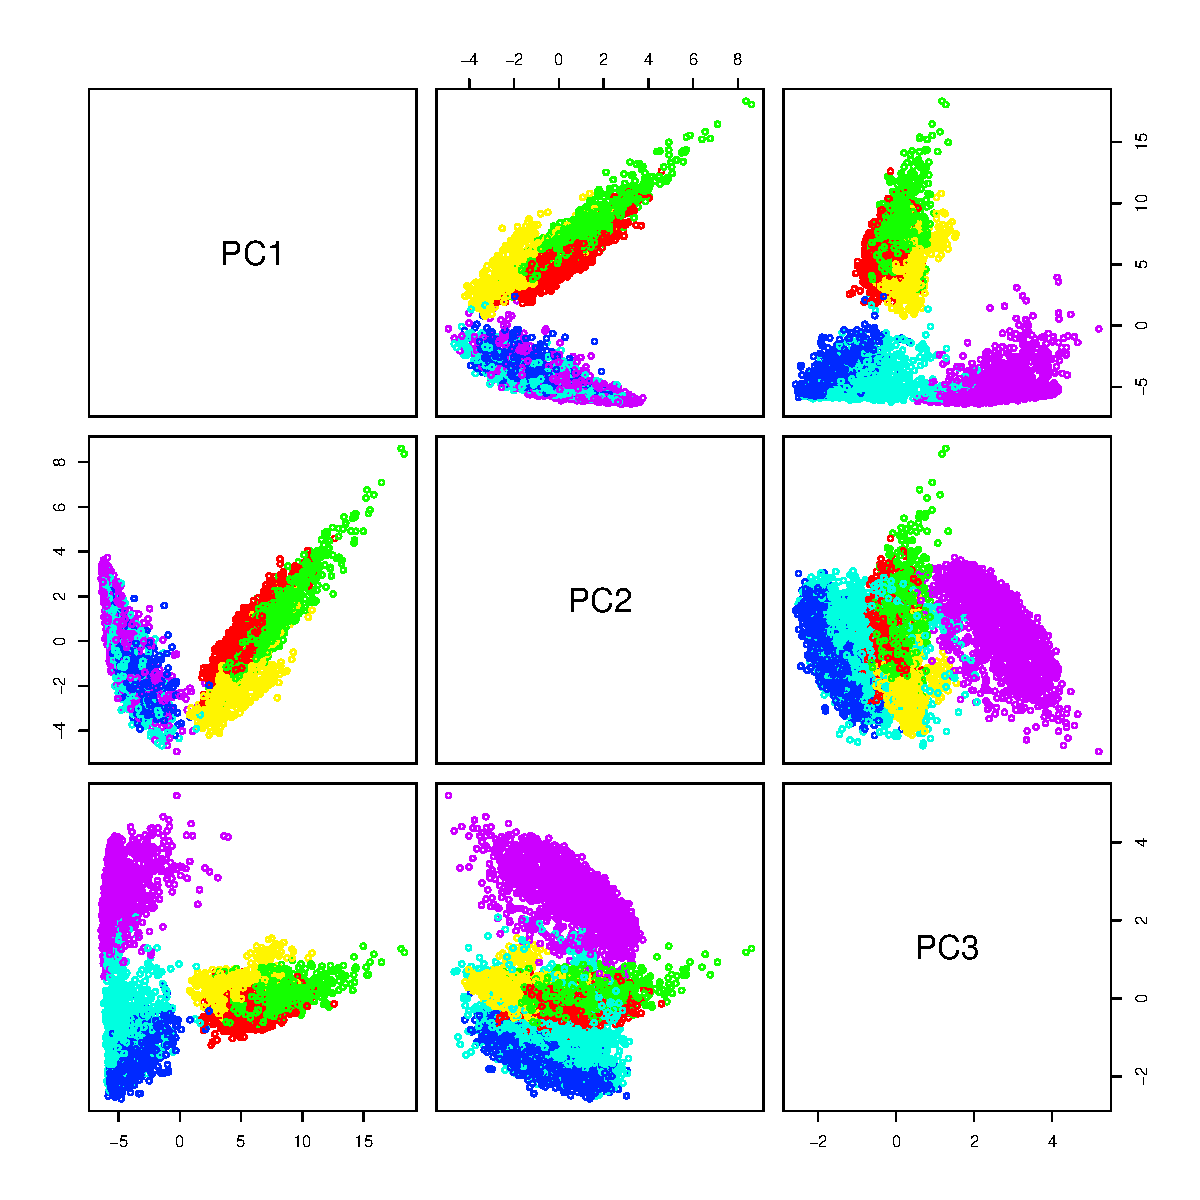
\includegraphics[width=3.2in]{figure4.pdf}
\caption{First three PCs scatter plot. Red=WK, yellow=WU, green=WD, light blue=SI, dark blue=ST, and purple=LD.
}
\label{fig_sim}
\end{figure}

\subsection{Factor Analysis}
We also compare each feature's loadings on the first five factors in Figure 5. We observe that the 561 features are well grouped. For the first factor, most important features are traditional statistical and signal processing features. It is expected as the dynamic movements generate much more active signals from the sensors. In \cite{he2008activity}, the author proved that auto-regression based features are better in separating dynamic activities than traditional statistical and frequency domain features. Therefore, auto-regression coefficients have most loadings on the second factor. In static activities, there is not much body movements but the accelerometer measures gravitational force permanently. Therefore, the important features are mostly gravity related in the third factor.

\begin{figure}[!ht]
\centering
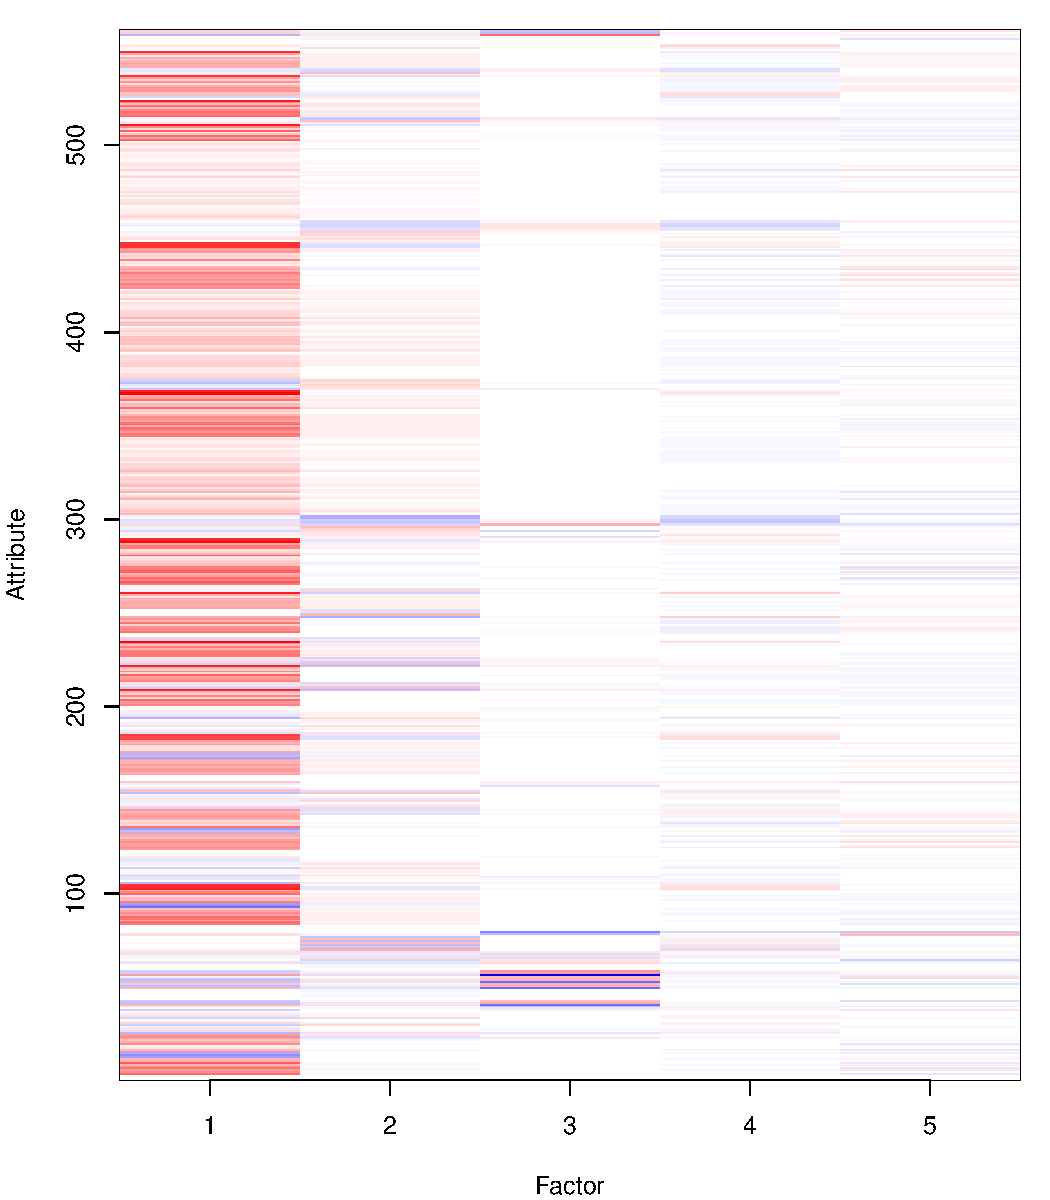
\includegraphics[width=2.8in]{figure5.pdf}
\caption{Each feature's weight on the first five factors. Red stands for large positive loading and blue stands for large negative loading.
}
\label{fig_sim}
\end{figure}

\section{Methodology}
In a multi-category classification problem, we are given a training dataset that consists of n samples $(\bm x_{i},y_{i})$ for $i=1,...,n$, where $\bm x_{i} \in R^{d}$ represents covariates and $y_{i} \in \{1,...,k\}$ denotes the class label of the sample. The task is to make a classification rule $\phi(\bm x): R^{d} \rightarrow \{1,...,k\}$ that well matches a feature $\bm x_{i}$ to a class label $y_{i}$.

In this Section, we discuss three well known classifiers, multiclass logistic regression, multiclass support vector machine and random forest.

\subsection{Multi-category Logistic Regression}
This widely-used method can be found in Chapter 5 of \citep{faraway2005extending}. 
We suppose that there are $K$ classes in response. For any pair ($i,K$), $i=1,2,...,K-1,$ we have:
$$\log\frac{P(Y=i|X=\bm x)}{P(Y=K|X=\bm x)}=\beta_{i0}+\bm\beta^{T}_{i}\bm x.$$
Thus, for any pair($i,j$), we have:
$$\log\frac{P(Y=i|X=\bm x)}{P(Y=j|X=\bm x)}=\beta_{i0}-\beta_{j0}+\bm\beta^{T}_{i}\bm x-\bm\beta^{T}_{l}.$$
The entire parameter set are:
$$\bm\theta=\{\beta_{10},\bm\beta_{1},\beta_{20},\bm\beta_{2},...,\beta_{(K-1)0},\bm\beta_{K-1}\}.$$
Under this assumption, the posterior probabilities are given by
$$P(Y=i|X=\bm x)=\frac{\exp(\beta_{i0}+\bm\beta^{T}_{i}\bm x)}{1+\sum^{K-1}_{l=1}\exp(\beta_{l0}+\bm\beta^{T}_{l}\bm x)},$$
for $i=1,2,...,K-1$, and
$$P(Y=K|X=\bm x)=\frac{1}{1+\sum^{K-1}_{l=1}\exp(\beta_{l0}+\bm\beta^{T}_{l}\bm x)}.$$
We want to maximize the conditional likelihood function, which is:
$$L(\bm\theta)=\sum^{n}_{k=1}\log(P(Y_k=y_k|X=\bm x_{k})).$$
After this, our classification rule is 
$$\phi(\bm x)=\text{argmax}_{i}{P(Y=i|X=\bm x)}.$$


\subsection{Multi-category Support Vector Machine}
Boser, Guon, and Vapnik (1992) introduced support vector machine (SVM). SVMs, which are available in both linear and nonlinear versions, involve optimization of a convex loss function under given constraints and so are unaffected by problems of local minima. This gives SVMs quite a strong competitive advantage over methods such as neural networks and decision trees.

For multi-category classification with k classes, $k>2$, we use the `one-against-one-approach'. We are going to train $k(k-1)/2$ binary classifiers using SVM and the appropriate class is found by a voting scheme. This means for an observation $x_m$, $1\leq m \leq n$, if one of those binary classifiers assign $x_m$ to a class $l$, $1 \leq l \leq k$, then we add one points to class $l$. At last, we will label $x_m$ to the class with highest score. If there are ties, we will do the multi-category classification again within the ties.

\subsection{Random Forest}
Breiman (2001) proposed random forest, which adds an additional layer of randomness to bagging. In addition to constructing each tree using a different bootstrap sample of the data, random forests change how the classification or regression trees are constructed.

The random forest algorithm (for both classification and regression) is as follows:
\begin{enumerate}
\item Draw $n_{tree}$ bootstrap samples from the original data.
\item For each of the bootstrap samples, grow an unpruned classification or regression tree, with the following modification: at each node, rather than choosing the best split among all predictors, randomly sample $m_{try}$ of the predictors and choose the best split from among those variables. (Bagging can be thought of as the special case of random forest obtained when $m_{try} = p$, the number of predictors.)
\item Predict new data by aggregating the predictions of the $n_{tree}$ trees (i.e., majority votes for classification, average for regression).
\end{enumerate}

\section{Results}
\subsection{Cross Validation}
Cross validation (CV) is an effective way to avoid model over-fitting. Through cross validation, we can select the best parameters to fit a model then apply to the testing data. In this project, we perform a 7-fold cross validation. In detail, we divide the 21 subjects in training set into 7 groups. For every group, we use the rest of 6 groups to train a model then predict it. There are several parameters to be considered:

\subsubsection{Number of PCs}
since there are 561 features in the dataset, then we have 561 PCs after PCA. For a typical prediction problem, more predictors often render better results. We observe that the misclassification rate decrease with more PCs. However, the computational cost increases as well. Moreover, the misclassification rates become unstable for logistic regression and SVM when the PCs number is larger than 100. Thus, we use 100 PCs for logistic regression and SVM and use the original 561 predictors for random forest.
\subsubsection{Kernel in SVM}
there are four typical kernels in SVM: linear, polynomial, radial, and sigmoid. By using the first 100 PCs, we find that the radial kernel with precision parameter (equivalent to the reciprocal of variance in the normal density) equal to 1/150 is the best kernel for this problem.
\subsubsection{$m_{try}$ in random forest}
  as mentioned in the previous section, $m_{try}$ is the number of predictors chosen for each split. By using the 561 predictors to fit the model, the best $m_{try}$ is 7.\\


Table II lists the CV results for those three classifiers by using the best parameters. The ``CV Error'' refers to the total misclassification rate. By comparing the results in Table II, the SVM outperforms the other two classifiers with 5.75$\%$ CV error.

\begin{table}[htbp]
% increase table row spacing, adjust to taste
\renewcommand{\arraystretch}{1.3}
\caption{Classifacation Performance}
\label{Classifacation Performance}
\centering
\begin{tabular}{ccc}
\hline\hline
Classifier&CV Error&Test Error\\
\hline
Logistic Regression&$8.8\%$&$5.84\%$\\
SVM&$5.75\%$&$3.81\%$\\
Random Forest&$7.34\%$&$6.17\%$\\
\hline\hline
\end{tabular}
\end{table}

\subsection{Performance}
The misclassification rates for the three models on testing dataset are also reported in Table II. First, we notice that the SVM is still the best model for this particular testing dataset. Second, we also find all the test errors are all smaller than CV errors, meaning that this testing dataset is a relatively easy splitting dataset compared to the general population.

The confusion matrix for SVM is also shown in Table 3. In Table 3, each row stands for the actual activity and each column stands for the predicted activity. The last column, error rate, also known as the true positive rate, measures the misclassification rate in each class.

\begin{table}[htbp]
\renewcommand{\arraystretch}{1.3}
\caption{Confusion Matrix for SVM}
\centering
\begin{tabular}{cccccccc}
\hline\hline
Activity&WK&WU&WD&SI&ST&LD&Sensitivity\\
\hline
WK&$493$&$0$&$3$&$0$&$0$&$0$&$0.61\%$\\
WU&$17$&$453$&$1$&$0$&$0$&$0$&$3.82\%$\\
WD&$1$&$8$&$411$&$0$&$0$&$0$&$2.14\%$\\
SI&$0$&$2$&$1$&$451$&$52$&$2$&$11.22\%$\\
ST&$0$&$0$&$0$&$27$&$529$&$0$&$4.86\%$\\
LD&$0$&$0$&$0$&$0$&$0$&$545$&$0.00\%$\\
\hline\hline
\end{tabular}
\end{table}

The SVM shows extraordinary performance in separating dynamic from static activities, and vice versa. There are only total of 3 incidents where the sitting activity is misclassified as dynamic activities. None of the dynamic activities are misclassified as one of the static activities. As shown in Table III, the dynamics activities show less misclassification rate than the static activities. It is mostly due the nature of the activities. Among these three dynamic activities, the human body accelerates in difference directions. For walking upstairs and downstairs, the human body accelerates in a complete opposite direction. Therefore, there is only 1 misclassification from walking upstairs to walking downstairs. Although walking upstairs and downstairs have distinct movement, but walking downstairs usually accelerates faster than walking upstairs as it is easier to walk downstairs than upstairs. Therefore, walking upstairs is more likely to be classified as walking straightforward. 

In static activities, there is high misclassification rate between sitting and standing. It could be due the experiment setup which the device is placed on the participant's waist. The device's orientation could be the same in both activities especially if the participant sits up very straight. In contrast, there is no misclassification incident for the lying down static activity. As the participant lies down, there orientation of the device is complete rotated by at least 90 degrees as compared to all other activities. It results significant different sensor readings for lying down.

\section{Conclusion}  
In this report, we study the smartphone based human activities dataset from UCI machine learning repository. The dataset includes 561 features extracted from the raw data collected from 30 participants. The goal is to predict human's activities (walking, walking downstairs, walking upstairs, standing, sitting, and lying) based on those 561 features. Although there is a very strong subject effect, we still have a large number of features with sufficient activity effect. It indicates that these 561 features are very useful in classifying the six activities. 

The principal component analysis and factor analysis show that the first three principle components (PCs) have an explicit interpretation. The first PC mainly splits the dynamic activities and static activities; the second PC along with the first PC helps in distinguishing dynamic activities; and the third PC is useful in differentiating static activities. The first 100 out of 561 PCs are used for classification for computational cost and accuracy balance. We propose and build three classifiers for classification: logistic regression, support vector machine, and random forest. The 7-fold cross validation shows that the SVM with radial kernel is the best model for this dataset.  Moreover, the SVM out performs the other two classifiers on the testing dataset with misclassification rate of $3.8\%$.


\bibliographystyle{plain}
\bibliography{project_report}

\end{document}